\chapter{METHODOLOGIES}

\graphicspath{ {./methodologies/} }
%%%%%%%% This line gets rid of page number on first page of text
\thispagestyle{empty}

%%%%%%%%%%%%%

\section{Method Selection}

The methodologies section covers methods chosen to investigate the research problem. We begin this section by restating our research problem and underlying assumptions underpinning our study: interpreting and understanding deep neural networks using interactive visualization, to inspire human curiosity and learning among the non-technical audience, as well as broaden people's access to interactive tools for deep learning.

\subsection{Scientific Methods}

The primary method selected for the research process is the scientific method. We selected this method as it involves careful observation and empirical study.

As deep learning is essentially a method for machines to learn from data and classifying patterns that is loosely modeled on the way a biological brain learns to solve problems. The scientific method is aptly suited for this type of research as it involves careful observation and empirical study of the topic in question, which includes rigorous skepticism about what is observed and iterative testing and experimentation to validate or invalidate it.

The underlying principles of the scientific method \cite{gauch_jr_2012} are essential for evaluating the hypothesis, enhancing perspective, increasing productivity, and inspiring innovation. These principles include logic, probability, parsimony and hypothesis testing, as well as science's presuppositions, limitations, principles and bold claims of rationality and truth. Beyond such methodology, some practical issues are shared broadly across the sciences, such as implementing effective science education and relating the scientific enterprise to the humanities.

The scientific method consists of two stages: the first consists of formulating hypotheses, and the second consists of testing them \cite{2016397}. What differentiates this from other forms of methods is the second stage: subjecting hypotheses to empirical testing by ascertaining whether or not predictions derived from hypotheses are borne out in relevant observations and experiments. Hypotheses and assumptions are the initial stages of scientific inquiry because they incentivize seeking truth and a hint as to where to find it \cite{AYALA2016xi}.

Additionally, we also employed other research methods to support our research processes, such as action as research, agile development and system design. The selection of a research methodology was dependent on the research question itself and how best it can be addressed: interpreting deep neural networks.

\subsection{Action Research}
Action Research is a research methodology driven by practical problems, emphasis participatory research, and develops practically useful solutions to a real-world problem iteratively. It offers a systematic, collaborative approach to conducting research that satisfies both the need for scientific rigor and promotion of sustainable social change and has been taken up by a variety of researchers in both academic and industrial settings \cite{Hayes:2011:RAR:1993060.1993065}.

Further, Action Research emphasizes the knowledge produced in the context of the application \cite{401014119781201}. It’s a distinct candidate research method when the objective is to explore theory concerning practice.

\section{Research Hypothesis}

While deep neural networks learn efficient and powerful representations and deliver superior performance, most users consider them as a ‘black-box.’ As in most cases, they learn representation and patterns that is difficult to extract and present it in a human-readable form. While this can be true for certain types of deep learning models, it is not entirely true for an image recognition model because they are representation of visual concepts which can be deconstructed to see what patterns were detected by the model at successive layers and how does that correlate to the prediction output.

\section{Design Goals}

\begin{figure}[htbp]
\centering
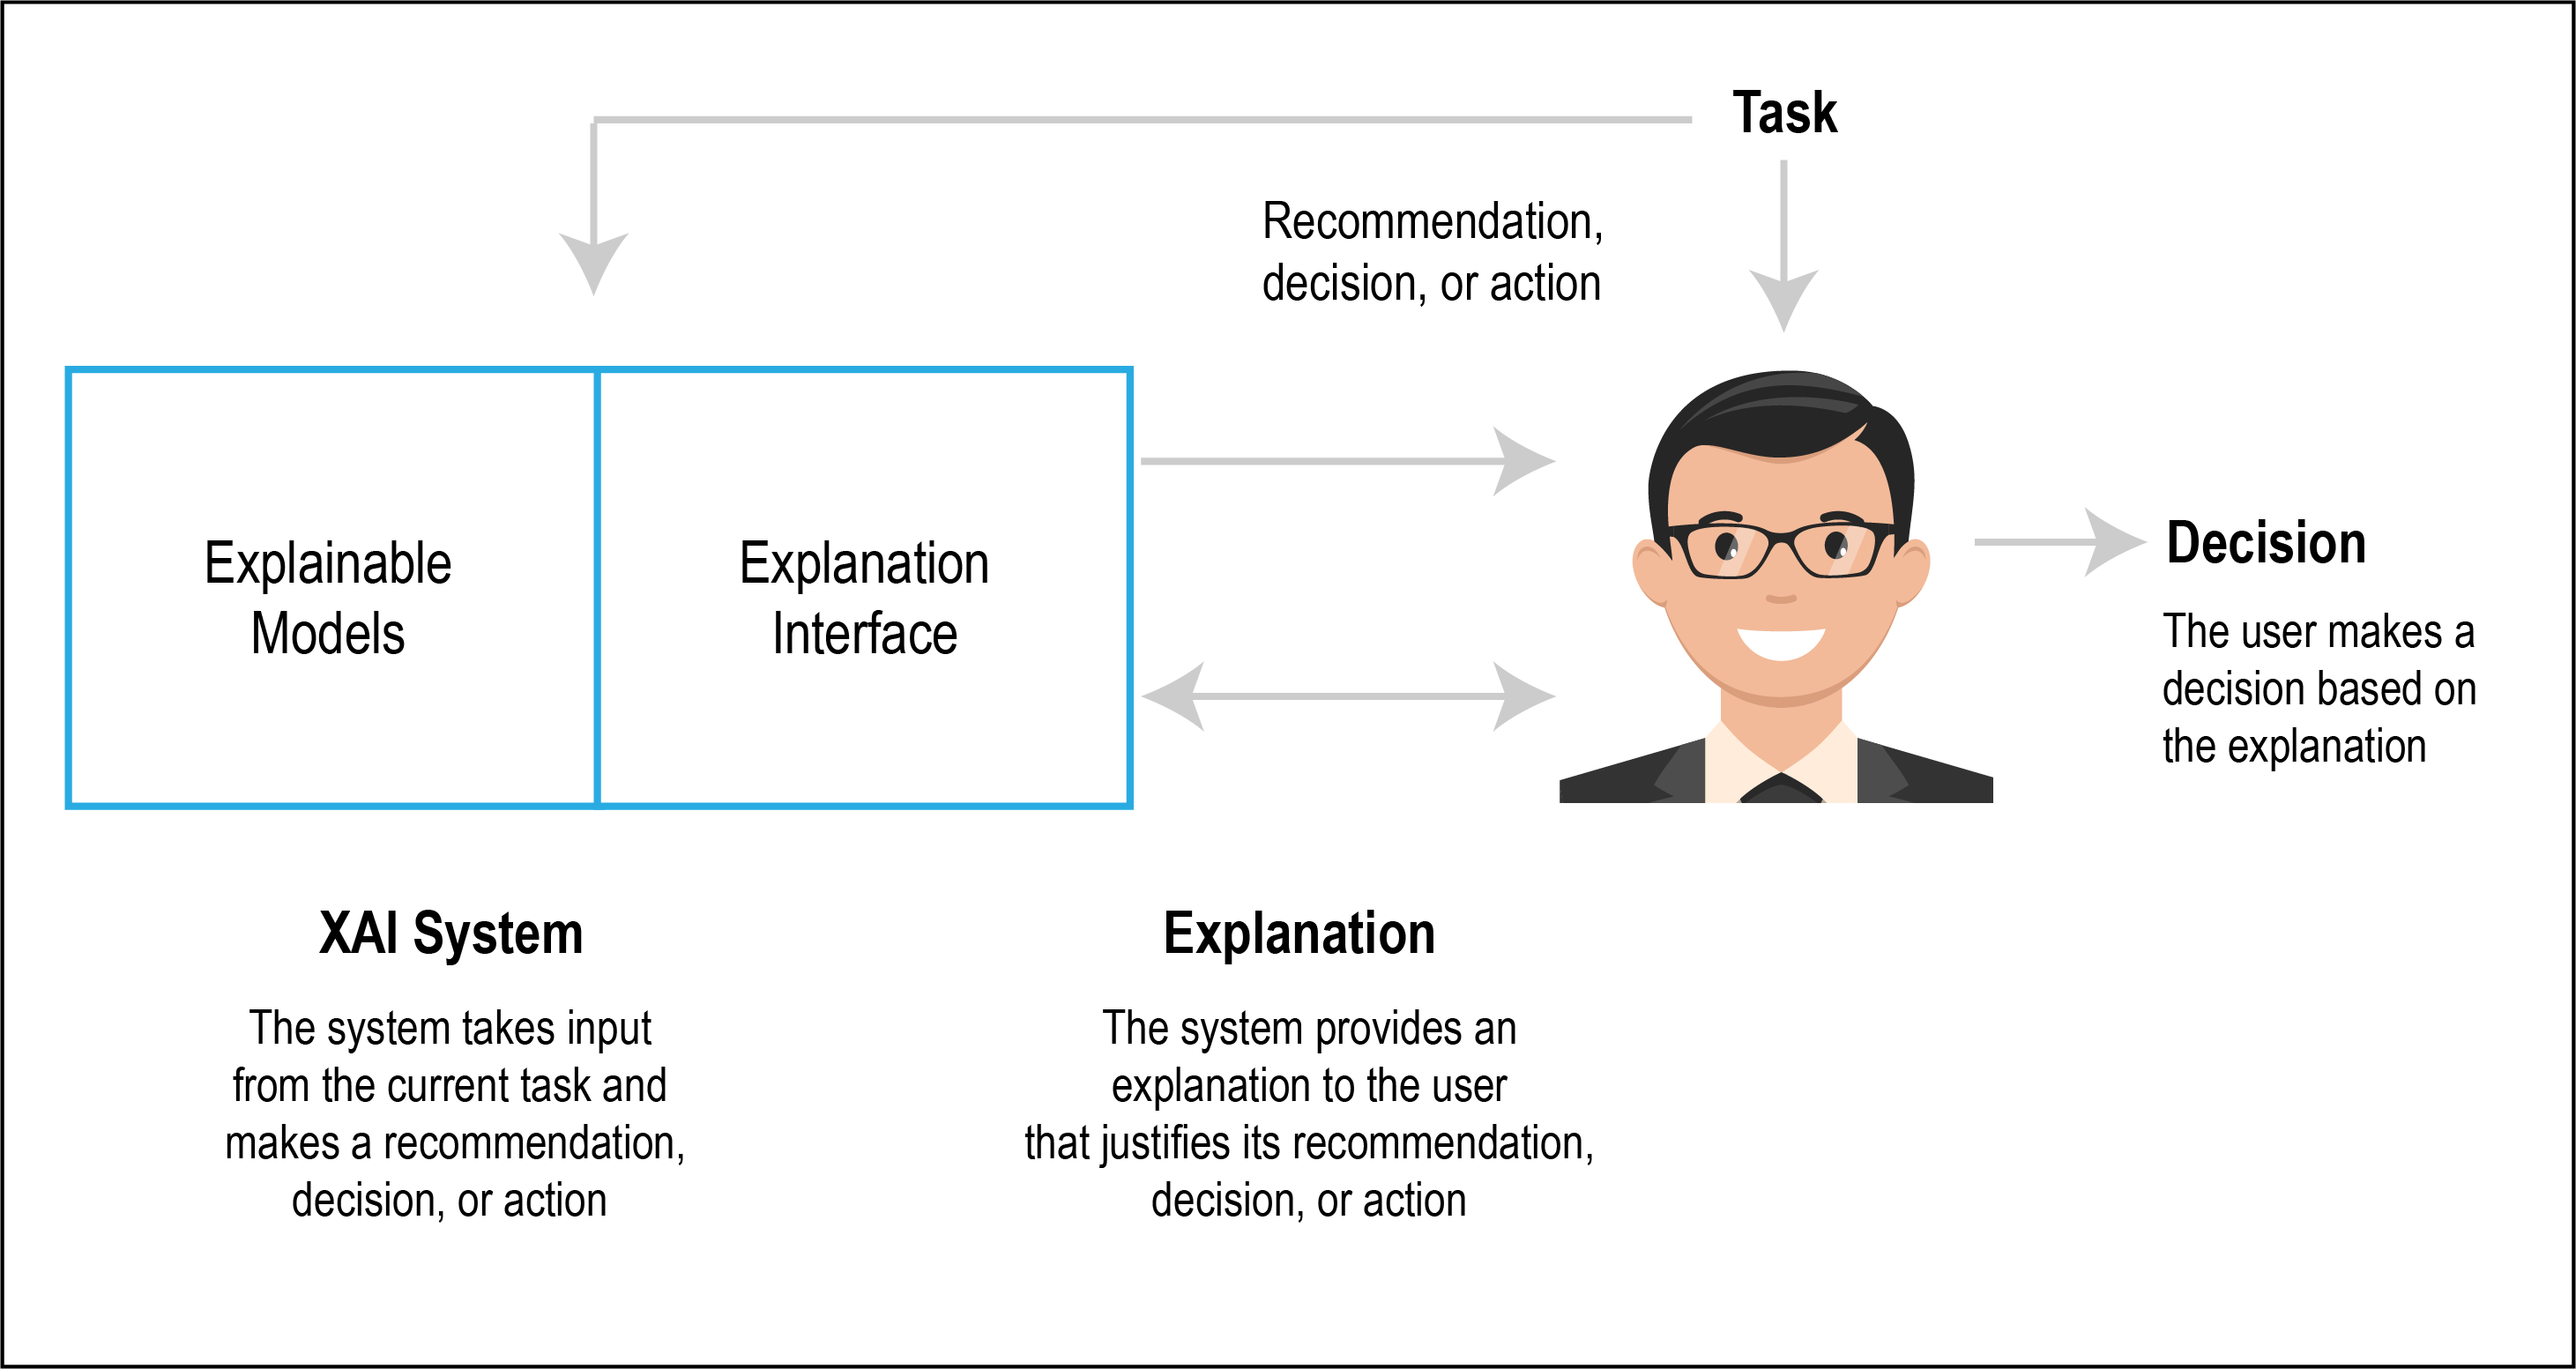
\includegraphics[width=1\textwidth]{images/xai-1-01.png}
\caption{Explanation Approach -> METHODOLOGIES}
\label{fig:explanation-approach}
\end{figure}

<REWRITE> Building upon our research question stated in the above section; we formulated our hypothesis as follows -  Develop a prototype that serves a set of utilities or toolkit for interpreting a visual classifier by providing visual evidence for their decision using interactive visualization.

Visualization is a potentially a powerful techniques to fill such a critical need of a black box. To deconstruct the inference process of an image model: 

We propose a visualization technique to understand neural net inference on a given image.  The representations learned by deep neural net like CNN are highly responsive to visualization, in large part because they are representations of visual concepts.

Motivated by the notion of explainablitiy and interpretable model 

localization in the context of CNNs, where the task is to localize objects in images using only whole image class labels

We would like to know what attributed to the classification decision.

Our work focuses on explaining decisions the network can possibly make using visual evidence 

***** TO OBTAIN THE LOCALIZATION MAP*****

A number of previous works have asserted that deeper representations in a CNN capture higher-level visual constructs [5, 35]. Furthermore, convolutional features naturally retain spatial information which is lost in fully-connected layers, so we can expect the last convolutional layers to have the best compromise between high-level semantics and detailed spatial information. The neurons in these layers look for semantic class-specific information in the image (say object parts). Grad-CAM uses the gradient information flowing into the last convolutional layer of the CNN to understand the importance of each neuron for a decision of interest. Although

our approach is the Class Activation Map-
ping (CAM) approach to localization [51]. This approach modifies image classification CNN architectures replacing fully-connected layers with convolutional layers and global average pooling [28], thus achieving class-specific feature maps. Others have investigated similar methods using global max pooling

We introduce a way of combining feature maps using the gradient signal.....

\section{Prototype Objective}
A client side deep learning application===
<REWRITE> The prototype is intended and designed for people with a non-technical background to understand the fundamental concepts of the neural network, in our case, a visual classifier. Our objective can be summarized mainly as (1) Explanation of neural networks for people with a non-computer science background (2) Inspire curiosity and learning among non-technical audiences  (3) Broadens people's access to interactive tools for deep learning.

\section{Technical Design}
The following segment provides an overview of the technical design and resources required for the successful development of the prototype. It provides a high-level overview of the components in scope, functionality, dataset and environmental setup.

\subsection{Client-side Neural Network}
Developing AI applications using modern deep learning framework is a non-trivial task. Normally these frameworks and libraries are leveraged by native applications that run on a native platform environment such as Linux, Windows, MacOS/iOS and Android. Thus most production-level libraries are developed for and written in Python, Java and C++. 

Developing AI application that is cross-platform and portable on multiple devices is not easy. The development of a native application is an intricate and time-consuming process. It is particularly complicated for mobile applications as the app vendors usually need to develop and maintain both iOS and Android version, in addition to the desktop application.

Compared to the native application, client-side applications can make the portability issue simpler for the cross-platform. The sample implementation of deep learning powered web application can be deployed on multiple platforms regardless of operating systems, hardware or device types.

Deep learning in the browser is at the experimental stage and recently a bunch of JavaScript-based deep learning framework has been introduced, making it possible to perform several deep learning tasks directly on the browser. Some of the supported features include model training, importing pre-trained models, transfer learning and inferences.

However, there is a debate on the feasibility and effectiveness of the web-based deep learning applications. One one hand, those who object think browsers are not primed for running deep learning tasks and its merely impractical due to the poor performance of client-side scripting and limitations imposed by the browsers. 

On the other hand, advocates think that the browser is an ideal platform for realizing client-side machine learning that allows highly rich interaction and improves personalization for end users. The benefits include but not limited to faster user interaction, preserving data privacy, lower back-end payload, reduced data transfer and performance latency of HTTP client-server communication.

\subsection{Supported Browser Features}
We analyzed the supported browser features for machine learning tasks and taken into consideration the factors that may affect the efficiency when building and deploying deep learning application on the web. One of them is the debugging capability to support model and data inspection when running deep learning tasks.

Further, in-browser deep learning allows users to use their local data and then train the model directly in the browser, which means there is no back-end end or server is necessary. 

\subsection{Model Selection}

As model selection is the centerpiece of the data science workflow, we evaluated a set of candidate pre-trained models by running a series of study and experiments. This also helped assess if the data collected for inference is suited to the problem of model selection. We taken into account the hyperparameter setting and other configuration details required to evaluate during the inference process if required. We tested the compatibility of the model with the available dataset. Based on our evaluation we selected VGG-16 as the primary model for the prototyping phase.

A schematic view of Visual Geometry Group 16 Model.~\ref{fig:CNN-2}.
\begin{figure}[htbp]
\centering
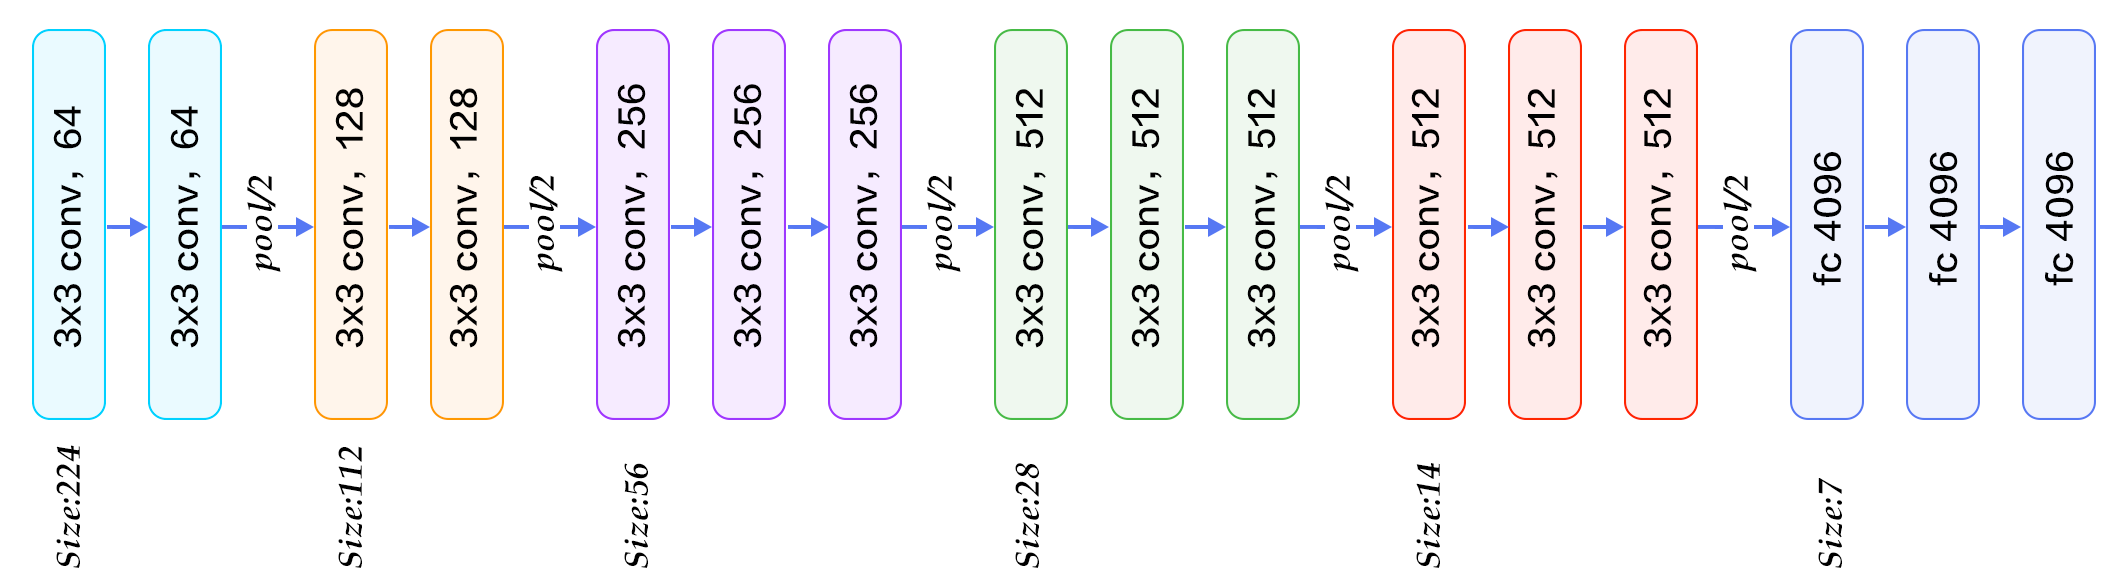
\includegraphics[width=1\textwidth]{images/cnn-vgg16-1.png}
\caption{VGG16 hidden layers}
\label{fig:CNN-2}
\end{figure}

VGG-16 is based on convolutional neural network model proposed by the Visual Geometry Group from the University of Oxford in the paper “Very Deep Convolutional Networks for Large-Scale Image Recognition” \cite{2014arXiv1409.1556S}. The model achieves 92.7\% top-5 test accuracy in ImageNet, which is a dataset of over 14 million images belonging to 1000 classes. It was one of the famous model submitted to ILSVRC-2014 competition. Ths list of hidden layers can be seen in the table \ref{table:vgg16-layer}. This model is used as the backbone network in our project.

\subsection{Dataset}

ImageNet is a massive database of image collection that consist of over 15 million labeled high-resolution images belonging to roughly 22,000 categories \cite{edsarx.1409.057520140101}. These images were downloaded from Google image search and labeled by humans using Amazon's Mechanical Turk crowd-sourcing tool in 2012. It took about two and half years to label all the images. 

The labeled dataset was first introduced in a competition called the ImageNet Large-Scale Visual Recognition Challenge (ILSVRC). The competition used a subset of ImageNet with around 1000 images in each of 1000 categories. In total, there are 1.2 million training images, 50,000 validation images, and 150,000 testing images. To maintain consistency of resolution, images have been down-sampled to a fixed resolution of 256x256 dimensions.
    
\subsection{Framework Selection}

To develop client-side deep learning application, we surveyed several open source machine learning framework for the web such as TensorFlow, Keras, and WebDNN. Based on our assessment and feedback from the developer community, we opted for TensorFlow in Python and TensorFlow.js for the prototype development, which is used along JavaScript ES6 in a Node.js environment. It seemed to be a right choice fit for training and inferring deep learning models on the browser. While several other open source JS platforms for machine learning have appeared in recent past, we found TensorFlow.js as feature-rich and well-documented when compared to other web libraries.

Furthermore, TensorFlow.js takes advantage of GPU processing power to accelerate deep learning tasks on browsers via WebGL \cite{Ma2019}, which is an important criteria for our tool that runs inference on a vision based model. WebGL is a back-end compute and a JavaScript API for rendering interactive 2D and 3D graphics within web browser without the use of additional plug-ins.

Since both client-side and server-side framework are part of the TensorFlow ecosystem, we can access APIs that are compatible with either ones. This also makes model conversion easier and allows for models to be ported between Python and JavaScript ecosystems \cite{Smilkov2019}.

\section{Environment Setup}
HPC Prince

\section{System Design}

As one of our goal for the prototype is to broaden people's access interactive tools for deep learning, and that the tool is targeted towards non-technical audience, DeepViz is a web-based interactive visualization tool that can be accessed from any modern web-browser. 

We setup the development environment for the client side application using JavaScript ecosystem and W3C web standards. DeepViz uses the web technologies: HTML, CSS, JavaScript ES6 and SVG. Node.js is used for back-end scripting for JavaScript ecosystem. We also use the Lucid library for experimenting and testing feature visualizations in VGG16 model

We leverage transpilers to transform code written in JavaScript ES6 into standard ES5 JavaScript that is executable in any browser. We also use bundling and tooling for local development and prototype deployment on the server.

We use SVG and D3.js for rendering vector graphics for the graph views. For the back-end deep learning framework, we executed all our code on an NVIDIA DGX, a workstation with 4 GPUs, with 16GB of RAM, 10 CPUs and 540GB of RAM.

\section{DeepViz - Visual Exploration Tool}

DeepViz is a visual exploration tool targeted towards the non-technical audience to explore the inference (or predictions) made by a visual classifier, an image recognition deep learning model.

it also enable developers to create interactive and explorable explanations for deep learning models on the web.

\iffalse
\section{Infrastructure and Tooling}
    \subsection{GPU Acceleration}
\subsection{Hardware}
\subsection{Software}
    \subsection{Build and Tooling}
\subsection{Cloud computing services}

    \subsection{Base Architecture}
    \subsection{Model Conversion}
    \subsection{Dataset}
    \subsection{Data Pre-processing}
    \subsection{Parameter Settings}
    \subsection{Application Prototype}
\subsection{Real-time processing}
\fi